\documentclass{article}

\usepackage{../packages}

\graphicspath{{./figures}}


\begin{document}
\begin{titlepage}
\begin{center}
	
\includegraphics[scale=0.7]{logo.png}

	\vspace*{4cm}
	\textbf{Bazy danych\\ Laboratorium}

	\vspace{1.5cm}
	\textit{Zapytania DDL SQL Oracle 2}

	\vspace{1.5cm}
	\textbf{Stanislau Antanovich}\\
	nr. indeksu: 173590\\
	gr. lab: L04

	\vspace{4.5cm}
\end{center}
\end{titlepage}

\tableofcontents
\listoffigures
\lstlistoflistings

\newpage
 
\section{Wprowadzenie}

\subsection{Cel ćwiczenia}

\subsection{Przygotowanie}

\section{Realizacja}

\begin{enumerate}
\item Tworzenie i wywołanie procedury \textbf{dodaj\_etat} pozwalającej na dodanie nowego etatu

\begin{lstlisting}[style=SQL, caption=\textit{Tworzenie i wywołanie procedury \textbf{dodaj\_etat}}]
CREATE PROCEDURE dodaj_etat(
	p_id IN NUMBER,
	p_etat IN VARCHAR
) AS
BEGIN
	INSERT INTO ETATY (ID_ETATU, ETAT) VALUES (p_id, p_etat);
	COMMIT;
END dodaj_etat;

EXEC dodaj_etat(673, 'EMPLOYEE')
\end{lstlisting}

		\begin{figure}[H]
			\centering
			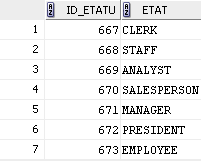
\includegraphics[scale=1.2]{zadanie1.png}
			\caption{\textit{Tworzenie i wywołanie procedury \textbf{dodaj\_etat}}}
		\end{figure}

\item Tworzenie i wywołanie procedury \textbf{usun\_pracownika} pozwalającej na usunięcie pracownika na podstawie podanego id(parametr wejściowy)

\begin{lstlisting}[style=SQL, caption=\textit{Tworzenie i wywołanie procedury \textbf{usun\_pracownika}}]
CREATE PROCEDURE usun_pracownika(
	id_pracownika IN NUMBER;
) AS
BEGIN
	DELETE FROM PRACOWNICY WHERE ID_PRACOWNIKA = id_pracownika;
END usun_pracownika;

EXEC usun_pracownika(7369);
\end{lstlisting}

		\begin{figure}[H]
			\centering
			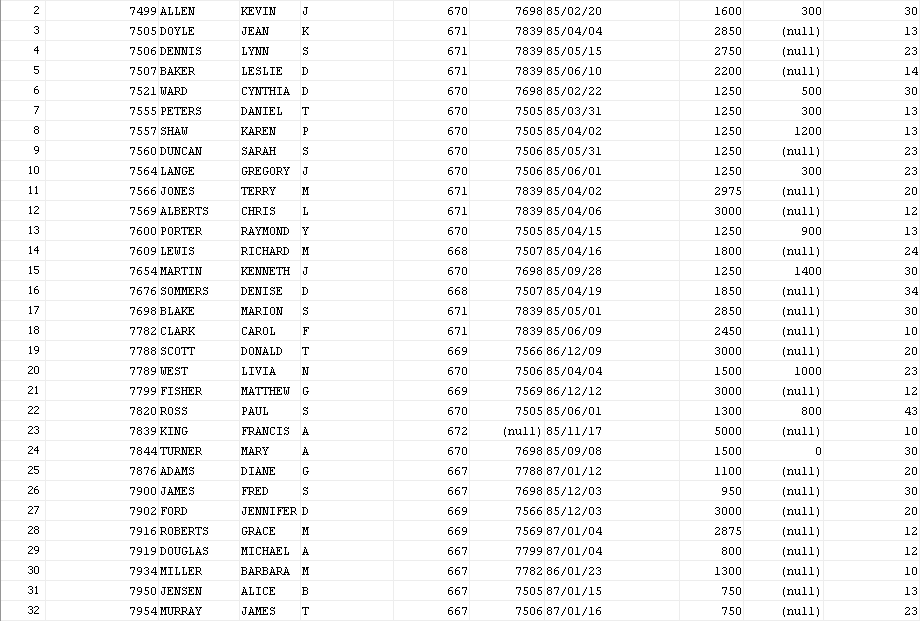
\includegraphics{zadanie2.png}
			\caption{\textit{Tworzenie i wywołanie procedury \textbf{usun\_pracownika}}}
		\end{figure}

\item Tworzenie i wywołanie proceduty \textbf{edytuj\_pracownika} pozwalającej na edytowanie kolumn pracownika na podstawie podanych parametrów

\begin{lstlisting}[style=SQL, caption=\textit{Tworzenie i wywołanie procedury \textbf{edytuj\_pracownika}}]
CREATE PROCEDURE edytuj_pracownika(
	id_pracownika IN NUMBER;
	nazwisko IN VARCHAR;
	imie IN VARCHAR;
	pensja IN NUMBER;
	prowizja IN NUMBER;
) AS
BEGIN
	UPDATE PRACOWNICY SET NAZWISKO = nazwisko, IMIE = imie, PENSJA = pensja, PROWIZJA = prowizja WHERE ID_PRACOWNIKA = id_pracownika;
END edytuj_pracownika

EXEC edytuj_pracownika(7499, 'ANTANOVICH', 'STANISLAU', 5000, 0);
\end{lstlisting}

		\begin{figure}[H]
			\centering
			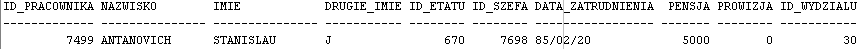
\includegraphics{zadanie3.png}
			\caption{\textit{Tworzenie i wywołanie procedury \textbf{edytuj\_pracownika}}}
		\end{figure}

\item Modyfikacja procedury \textbf{dodaj\_etat} w taki sposób, aby uniknąć wystąpienia duplikującego się rekordu.

\begin{lstlisting}[style=SQL, caption=\textit{Modyfikacja procedury \textbf{dodaj\_etat}}]
CREATE PROCEDURE dodaj_etat(
	id_etatu IN NUMBER,
    	etat IN VARCHAR
) AS etat_count NUMBER;
BEGIN
	SELECT COUNT(*) INTO etat_count FROM ETATY WHERE ID_ETATU = id_etatu;
	IF etat_count = 0 THEN
		INSERT INTO ETATY (ID_ETATU, ETAT)
		VALUES (id_etatu, etat);
		COMMIT;
	END IF;
END dodaj_etat;
/

EXEC dodaj_etat(666, 'NOWY ETAT');
\end{lstlisting}

		\begin{figure}[H]
			\centering
			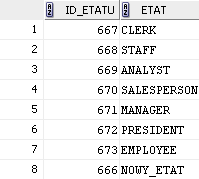
\includegraphics{zadanie4.png}
			\caption{\textit{Modyfikacja procedury \textbf{dodaj\_etat}}}
		\end{figure}

\item Zaproponowana funkcja \textbf{srednia\_pensja}, która zwraca średnią pensję wszystkich pracowników
	
\begin{lstlisting}[style=SQL, caption=\textit{Zaproponowana funckja \textbf{srednia\_pensja}}]
CREATE FUNCTION srednia_pensja RETURN NUMBER
IS
	avg_pensja NUMBER;
BEGIN
	SELECT AVG(PENSJA) INTO avg_pensja FROM PRACOWNICY;
	RETURN avg_pensja;
END srednia_pensja;
/

SELECT srednia_pensja() FROM DUAL;
\end{lstlisting}

		\begin{figure}[H]
			\centering
			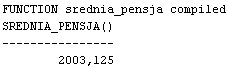
\includegraphics[scale=1.2]{zadanie5.png}
			\caption{\textit{Zaproponowana funkcja \textbf{srednia\_pensja}}}
		\end{figure}

\item Zaproponowana funkcja \textbf{zmien\_prowizje}, która umożliwi na podstawie id pracownika zmienić jego prowizję. W przypadku wprowadzonej wartości poniżej zera funkcja ma zgłosić odpowiedni wyjątek

\begin{lstlisting}[style=SQL, caption=\textit{Zaproponowana funkcja \textbf{zmien\_prowizje}}]
CREATE FUNCTION zmien_prowizje(
	id_pracownika IN NUMBER,
	prowizja IN NUMBER
) RETURN VARCHAR
IS
BEGIN
	IF prowizja < 0 THEN
		RAISE_APPLICATION_ERROR(-20001, 'Prowizja nie moze byc ponizej zera')
	ELSE
		UPDATE PRACOWNICY SET PROWIZJA = prowizja WHERE ID_PRACOWNIKA = id_pracownika;
		COMMIT;
		RETURN 'Prowizja zostala zmieniona'
	END IF;
END zmien_prowizje;

DBMS_OUTPUT.PUT_LINE(zmien_prowizje(7499, 2000));
\end{lstlisting}

	\begin{figure}[H]
		\centering
		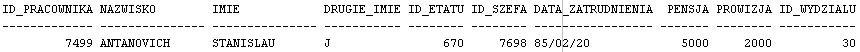
\includegraphics{zadanie6.png}
		\caption{\textit{Zaproponowana funkcja \textbf{zmien\_prowizje}}}
	\end{figure}

\item Zaproponowana funkcja \textbf{ilosc\_pracownicy\_z\_pensja} umożliwiająca zwrócenie ilości pracowników, których pensja mieści się w podanym przedziale <min;max>

\begin{lstlisting}[style=SQL, caption=\textit{Zaproponowana funkcja \textbf{ilosc\_pracownicy\_z\_pensja}}]
CREATE FUNCTION ilosc_pracownicy_z_pensja(
	min_pensja IN NUMBER,
	max_pensja IN NUMBER
) RETURN NUMBER
IS
	e_count NUMBER;
BEGIN
	SELECT COUNT(*) INTO e_count FROM PRACOWNICY WHERE PENSJA BETWEEN min_pensja AND max_pensja;
	RETURN e_count;
END ilosc_pracownicy_z_pensja;
/

SELECT ilosc_pracownicy_z_pensja(1000,2500) FROM DUAL;
\end{lstlisting}

	\begin{figure}[H]
		\centering
		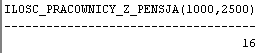
\includegraphics[scale=1.2]{zadanie7.png}
		\caption{\textit{Zaproponowana funkcja \textbf{ilosc\_pracownicy\_z\_pensja}}}
	\end{figure}

\item Zaproponowana funkcja \textbf{zwieksz\_pensje}, która na podstawie id pracownika zmienia wartość kolumny pensja zgodnie z zasadami:
\begin{itemize}
\item jeżeli pracownik nie ma zwierzchnika jego pensja nie ulega zmianie
\item jeżeli pracownik ma zwierzchnika, ale ma prowizje, pensja zwiększa się o wartość 100
\item jeżeli pracownik ma zwierzchnika, ale nie ma prowizji, pensja zwiększa się o 10\%
\item funkcja zwraca nową pensję jako wartość
\end{itemize}

\begin{lstlisting}[style=SQL, caption=\textit{Zaproponowana funkcja \textbf{zwieksz\_pensje}}]

CREATE FUNCTION zwieksz_pensje(
	id_pracownika IN NUMBER
) RETURN NUMBER
IS
	pensja NUMBER;
	z_pensja NUMBER;
	prowizja NUMBER;
BEGIN
	SELECT PENSJA, PROWIZJA INTO pensja, prowizja FROM PRACOWNICY WHERE ID_PRACOWNIKA = id_pracownika;
	IF prowizja IS NULL THEN
	SELECT PENSJA INTO z_pensja FROM PRACOWNICY WHERE ID_PRACOWNIKA = (SELECT ID_SZEFA FROM PRACOWNICY WHERE ID_PRACOWNIKA = id_pracownika) FETCH FIRST ROW ONLY;
	pensja := pensja * 1.1;
		IF z_pensja IS NOT NULL THEN
			pensja := pensja + 100;
		END IF;
	ELSE
		pensja := pensja + 100;
	END IF;

	UPDATE PRACOWNICY SET PENSJA = pensja WHERE ID_PRACOWNIKA = id_pracownika;
	COMMIT;
	RETURN pensja;
END zwieksz_pensje;
/

SELECT zwieksz_pensje(7499) FROM DUAL;
\end{lstlisting}

\begin{figure}[H]
	\centering
	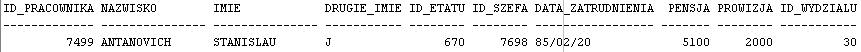
\includegraphics{zadanie8.png}
	\caption{\textit{Zaproponowana funkcja \textbf{zwieksz\_pensje}}}
\end{figure}

\item Wywołanie komendy usunięcia dowolnej procedury i funkcji
	
\begin{lstlisting}[style=SQL, caption=\textit{Wywołanie komendy usunięcia dowolnej procedury i funkcji}]
DROP PROCEDURE dodaj_etat;
\end{lstlisting}

	\begin{figure}[H]
		\centering
		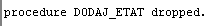
\includegraphics[scale=1.4]{zadanie9.png}
		\caption{\textit{Wywołanie komendy usunięcia dowolnej procedury i funkcji}}
	\end{figure}

\item Zaproponowany typ pozwalający przechowywać dane obiektu \textbf{ETAT} oraz tabelę etatów

\begin{lstlisting}[style=SQL, caption=\textit{Zaproponowany typ pozwalający przechowywać dane obiektu \textbf{ETAT} oraz tabelę etatów}]
CREATE TYPE typ_etat AS OBJECT (
	id_etatu NUMBER,
	etat VARCHAR(255)
);
/

CREATE TYPE tabela_etatow AS TABLE OF typ_etat;
/
\end{lstlisting}
	
	\begin{figure}[H]
		\centering
		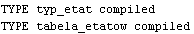
\includegraphics[scale=1.2]{zadanie10.png}
		\caption{\textit{Zaproponowany typ pozwalający przechowywać dane obiektu \textbf{ETAT} oraz tabelę etatów}}
	\end{figure}

\end{enumerate}

\section{Wnioski}

W wyniku przeprowadzonych działań udało mi się efektywnie wykorzystać narzędzie SQL Developer do zarządzania bazą danych. W ramach zadania, stworzyłem i wywołałem szereg procedur oraz funkcji, które umożliwiły mi dodawanie, usuwanie i edycję danych pracowników oraz etatów zgodnie z określonymi regułami.

Zaimplementowałem procedury takie jak dodaj\_etat, usuń\_pracownika oraz edytuj\_pracownika, które pozwoliły na manipulację danymi w sposób kontrolowany i bezpieczny. Modyfikując procedurę dodaj\_etat, zabezpieczyłem ją przed dodaniem duplikujących się rekordów, co przyczyniło się do poprawy integralności danych.

Dodatkowo, zaproponowałem funkcje takie jak srednia\_pensja, zmien\_prowizje, ilosc\_pracownicy\_z\_pensja oraz zwieksz\_pensje, które umożliwiły mi wykonywanie różnorodnych operacji na danych pracowników zgodnie z założeniami biznesowymi.

Pracując nad rozwojem funkcjonalności, wprowadziłem także definicje typu typ\_etat oraz tabela\_etat\_typ, co umożliwiło mi przechowywanie i manipulowanie danymi dotyczącymi etatów w bardziej strukturalny sposób.

W rezultacie przeprowadzonych działań, zdobyłem nowe umiejętności w obszarze zarządzania bazami danych oraz programowania w języku SQL. Wdrażając te rozwiązania, podjąłem skuteczne kroki w kierunku optymalizacji procesów związanych z zarządzaniem danymi w organizacji.

\end{document}
